\insertCompetition{11/10/18} {Ruckus at the Rock}{match.jpg}{driveteam.jpg}{16th} 
{

	\bigskip

	\textbf{Robot:}  Our hanging mechanism may have been slightly too ambitious for our first meet, because even though it was elegant and innovative, we were unable to make it work for the competition. We also focused too much of our time on the hanging mechanism, so we had a very basic collection mechanism that could only deposit in the depot. We had some minor success after taking off the hanging mechanism, which made our robot short enough to fit under the lander and much faster. This taught us that sometimes it is a good strategy to remove parts of the robot that are nonfunctional if it provides some other advantage, and it may be a good strategy to make our robot shorter so it can more easily navigate the field.

	\bigskip

	\textbf{Competition:} We need a more detailed checklist and more focus on packing. We forgot many integral things which made the competition more difficult and more stressful than it should have been, including the team marker and controller board. We made a list of things we forgot to improve our packing checklist and ensure that next time we double check that everything on the list is packed. Our scouting team was successful in gathering valuable information about the other teams, so we will continue with that method, most likely with newer members so they can learn how to do it. 

	\bigskip

	\textbf{General:} We need a more detailed schedule for when we want to achieve our goals, especially for when we want to complete certain parts of the robot. While we did plan to finish things far enough in advance to build in time for programming and driver practice, we ultimately did not achieve these goals and left ourselves with too little time to achieve as much as we had hoped to for the competition.

	\bigskip

	\textbf{Goals for Upcoming Qualifiers:} Finish building it at least 2 weeks before the competition so that it can be programmed and the drivers can have time to practice.

	\bigskip

	\textbf{Administrative:} Because of the issues we faced with completing the necessary work by the intended time, we will be using Trello, our project management app, to a larger extent. This means members will need to claim a task on Trello at the beginning of each meeting, ensuring everyone is working. Also, goals for when tasks should be finished will be put on both Trello and Band to hold people accountable to their goals.

	\bigskip

	\textbf{Robot:} We need to redesign our hanging mechanism to be stronger, easier to use, and more reliable, which will likely require a total change in concept. We also need a more effective method for collecting and scoring minerals into the lander. We are currently considering using an arm to extend into the crater to save time, but need to consider different methods of collection, such as rubber bands or surgical tubing. Finally, we must decide if we want to reach into the crater with an arm or drive in. If we are driving in, we need a new drivetrain, as our current one had trouble getting over the crater wall.

	\bigskip

	\textbf{Long-term Goals:} We must win 8 matches in our next 2 competitions to remain competitively viable in the League Championship, which increase our chances of moving on to States.

	\bigskip

	Unfortunately we didn’t perform as well as we had hoped to at our first meet. Our hang mechanism broke after practicing hanging off of the playing field and we had multiple problems with our code. We finished the day 16th with 2 wins and 4 losses. While we had many issues day of the competition, this was a great learning opportunity for everyone on our team. We plan to work on our time management and improving our designs with more prototyping and testing.
}
{
  \begin{itemize}
      \item Test software changes multiple times before matches; don't make sudden changes to the program before a match without testing
      \item Leave a full week after hardware and software changes for realistic and thorough driver practice to prepare drivers completely for the competition
      \item Practice the transition between the autonomous and teleop period 
      \item Keep multiple RC and DS phones fully charged for the day of the competition
      \item Keep some essential tools from the pits in a portable case along with the pits checklist 
  \end{itemize} 
}
{Rockledge High School, Rockledge, Fl}
\begin{figure}[ht]
  \centering
  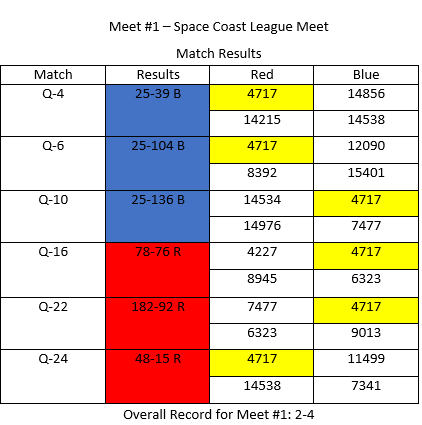
\includegraphics[width=0.9\textwidth]{Competition/Images/Meet1Score.PNG}
  \caption{}
  \label{fig:comparinggears}
\end{figure} 
\interesting{Our first meet at Rockledge High School}{competition:1}